
\section{Examples}
\label{sect:examples}

This section lists a number of examples of the types of operations that can be
performed with SeqPig.  Of course, what can be done is not limited to these
operations.

\subsection{Operations on BAM files}

To access sequencing data in BAM files, SeqPig uses Hadoop-BAM, which provides
access to all fields and optional attributes in the data records.

%Hadoop-BAM
%provides access to sequencing data in BAM and SAM format
%through the SAMRecord (see \url{http://picard.sourceforge.net/javadoc/net/sf/samtools/SAMRecord.html}),
%which is the Picard type for a (typically aligned) read. As such, all fields and
%optional attributes become accessible from within Pig.

All the examples below assume that an input BAM file is initially imported to HDFS via
\begin{lstlisting} 
prepareBamInput.sh input.bam
\end{lstlisting} 
and then loaded in the grunt shell via
\begin{lstlisting} 
A = load 'input.bam' using BamUDFLoader('yes');
\end{lstlisting} 
The 'yes' parameter to {\tt BamUDFLoader} chooses read attributes to be loaded; choose 'no' whenever these
are not required).

Once some operations have been performed, the resulting (modified) read
data can then be stored into a new BAM file via
\begin{lstlisting}
store A into 'output.bam' using BamUDFStorer('input.bam.asciiheader');
\end{lstlisting}
and can also be exported from HDFS to the local filesystem via
\begin{lstlisting}
prepareBamOutput.sh output.bam
\end{lstlisting}
\begin{description}
	\item[Note] the Pig store operation requires a valid header for the BAM output file,
for example the header of the source file used to generate it, which is
generated automatically by the {\tt prepareBamInput.sh} script used to import it)
\end{description}

Writing the BAM data to the screen (similarly to samtools view)
can be done simply by
\begin{lstlisting}
dump A;
\end{lstlisting}
Another very useful Pig command is {\tt describe}, which returns the schema that Pig
uses for a given data bag. Example:
\begin{lstlisting}
A = load 'input.bam' using BamUDFLoader('yes');
describe A;
\end{lstlisting}
returns
\begin{lstlisting}  
	BamData: {name: chararray,start: int,end: int,read: chararray,cigar: chararray,
   basequal: chararray,flags: int,insertsize: int,mapqual:int,matestart: int,
   materefindex: int,refindex: int,refname: chararray,attributes: map[]}
\end{lstlisting}
Notice that all fields except the attributes are standard data types (strings
or integers). Specific attributes can be accessed via {\tt attributes\#'name'}. For
example,
\begin{lstlisting} 
B = FOREACH A GENERATE name, attributes#'MD';
dump B;
\end{lstlisting}
will output all read names and their corresponding MD tag.
Other useful commands are {\tt LIMIT} and {\tt SAMPLE}, which can be used to
select a subset of reads from a BAM/SAM file.
\begin{lstlisting} 
B = LIMIT A 20;
\end{lstlisting}
will assign the first 20 records of A to B, while
\begin{lstlisting}
B = SAMPLE A 0.01;
\end{lstlisting}
will sample from A with sampling probability 0.01.

\subsubsection{Filtering out unmapped reads and PCR or optical duplicates}
Since the {\tt flags} field of a SAM record is exposed to Pig, one can simply
use it to filter out all tuples (i.e., SAM records) that do not have the
corresponding bit set.
\begin{lstlisting}
A = FILTER A BY (flags/4)%2==0 and (flags/1024)%2==0;
\end{lstlisting}
For convenience SeqPig provides a set of filters that allow a direct access
to the relevant fields. The previous example is equivalent to
\begin{lstlisting}
run scripts/filter_defs.pig
A = FILTER A BY not ReadUnmapped(flags) and not IsDuplicate(flags);
\end{lstlisting}
For of a full list of the available filters look at the file {\tt scripts/filter\_defs.pig}.

\subsubsection{Filtering out reads with low mapping quality}

Other fields can also be used for filtering, for example the read
mapping quality value as shown below.
\begin{lstlisting}
A = FILTER A BY mapqual > 19;
\end{lstlisting}

\subsubsection{Filtering by regions (samtools syntax)}

SeqPig also supports filtering by samtools \emph{region} syntax.
The following examples selects base positions 1 to 44350673
of chromosome 20.
\begin{lstlisting}
 DEFINE myFilter CoordinateFilter('input.bam.asciiheader','20:1-44350673');
 A = FILTER A BY myFilter(refindex,start,end);
\end{lstlisting}
Note that filtering by regions requires a valid SAM header for mapping
sequence names to sequence indices. This file is generated automatically
when BAM files are imported via the {\tt prepareBamInput.sh} script.

\subsubsection{Sorting BAM files}
Sorting an input BAM file by chromosome, reference start coordinate, strand
and readname (in this hierarchical order):
\begin{lstlisting}
A = FOREACH A GENERATE name, start, end, read, cigar, basequal, flags, insertsize,
mapqual, matestart, materefindex, refindex, refname, attributes, (flags/16)%2;
A = ORDER A BY refname, start, $14, name;
\end{lstlisting}
\begin{description}
	\item[Note] This is roughly equivalent to executing from the command line
\begin{lstlisting}
$ pig -param inputfile=input.bam -param outputfile=input_sorted.bam ${SEQPIG_HOME}/scripts/sort_bam.pig
\end{lstlisting}
\end{description}

 \subsubsection{Computing read coverage}
Computing read coverage over reference-coordinate bins of a fixed size,
for example:
\begin{lstlisting}
B = GROUP A BY start/200;
C = FOREACH B GENERATE group, COUNT(A);
dump C; 
\end{lstlisting}
will output the number of reads that lie in any non-overlapping bin of size 200 base pairs.

 \subsubsection{Computing base frequencies (counts) for each reference coordinate}
\begin{lstlisting}
A = FOREACH A GENERATE read, flags, refname, start, cigar, basequal, mapqual;
A = FILTER A BY (flags/4)%2==0;
RefPos = FOREACH A GENERATE ReadRefPositions(read, flags, refname, start, cigar, basequal), mapqual;
flatset = FOREACH RefPos GENERATE flatten($0), mapqual;
grouped = GROUP flatset BY ($0, $1, $2);
base_counts = FOREACH grouped GENERATE group.chr, group.pos, group.base, COUNT(flatset);
base_counts = ORDER base_counts BY chr,pos;
store base_counts into 'input.basecounts';
\end{lstlisting}
\begin{description}
	\item[Note] This is roughly equivalent to executing from the command line
\begin{lstlisting}
$ pig -param inputfile=input.bam -param outputfile=input.basecounts -param pparallel=1 ${SEQPIG_HOME}/scripts/basefreq.pig 
\end{lstlisting}
\end{description}

\subsubsection{Pileup}
Generating samtools compatible pileup (for a correctly sorted BAM file
with MD tags aligned to the same reference, should produce the same output as
{\tt samtools mpileup -A -f ref.fasta -B input.bam}):
\begin{lstlisting}
A = load 'input.bam' using BamUDFLoader('yes');
B = FILTER A BY (flags/4)\%2==0 and (flags/1024)\%2==0;
C = FOREACH B GENERATE ReadPileup(read, flags, refname, start, cigar,
      basequal, attributes#'MD', mapqual), start, flags, name;
C = FILTER C BY $0 is not null;
D = FOREACH C GENERATE flatten($0), start, flags, name;
E = GROUP D BY (chr, pos);
F = FOREACH E { G = FOREACH D GENERATE refbase, pileup, qual, start,
      (flags/16)\%2, name; G = ORDER G BY start, $4, name; GENERATE group.chr,
      group.pos, PileupOutputFormatting(G, group.pos); }
G = ORDER F BY chr, pos;
H = FOREACH G GENERATE chr, pos, flatten($2);
store H into 'input.pileup' using PigStorage('\t');
\end{lstlisting}
\begin{description}
	\item[Note] This is equivalent to executing from the command line
\begin{lstlisting}
$ pig -param inputfile=input.bam -param outputfile=input.pileup -param pparallel=1
    ${SEQPIG_HOME}/scripts/pileup.pig
\end{lstlisting}
\end{description}
The script essentially does the following:
\begin{enumerate}
\item Import BAM file and filter out unmapped or duplicate reads ({\tt A, B})
\item Break up each read and produce per-base pileup output ({\tt C, D})
\item Group all thus generated pileup output based on a (chromosome, position)
coordinate system ({\tt E})
\item For each of the groups, sort its elements by their position, strand and name;
then format the output according to samtools ({\tt F})
\item Sort the final output again by (chromosome, position) and perform
some Pig operation by unnesting tuples ({\tt G, H})
\item Store the output to a directory inside HDFS (last line)
\end{enumerate}
There are two optional parameters for pileup.pig: {\tt min\_map\_qual} and
{\tt min\_base\_qual} (both with default value 0) that filter out reads with
either insufficient map quality or base qualities. Their values can
be set the same way as the other parameters above.

There is an alternative pileup script which typically performs better but
is more sensitive to additional parameters. This second script, {\tt
pileup2.pig}, is based on a \emph{binning} of the reads according to
intervals on the reference sequence. The pileup output is then generated on
a by-bin level and not on a by-position level. This script can be invoked
with the same paramters as {\tt pileup2.pig}. However, it has tunable
parameters that determine the size of the bins ({\tt binsize}) and the
maximum number of reads considered per bin ({\tt reads\_cutoff}), which is
similar to the maximum depth parameter that samtools accepts. However,
note that since this parameter is set on a per-bin level you may chose it dependent on
the read length and bin size, as well as the amount of memory available on
the compute nodes.


\subsubsection{Collecting read-mapping-quality statistics}
In order to evaluate the output of an aligner, it may be useful to
consider the distribution of the mapping quality over the collection of
reads. Thanks to Pig's {\tt GROUP} operator this is fairly easy.
\begin{lstlisting}
A = load 'input.bam' using BamUDFLoader('yes');
B = FILTER A BY (flags/4)\%2==0 and (flags/1024)\%2==0;
read_stats_data = FOREACH B GENERATE mapqual;
read_stats_grouped = GROUP read_stats_data BY mapqual;
read_stats = FOREACH read_stats_grouped GENERATE group, COUNT($1);
read_stats = ORDER read_stats BY group;
STORE read_stats into 'mapqual_dist.txt';
\end{lstlisting}
\begin{description}
	\item[Note] This is equivalent to executing from the command line
\begin{lstlisting}
$ pig -param inputfile=input.bam -param outputfile=mapqual_dist.txt ${SEQPIG_HOME}/scripts/read_stats.pig
\end{lstlisting}
\end{description}

\subsubsection{Collecting per-base statistics of reads}
Sometimes it may be useful to analyze a given set of reads for a bias
towards certain bases being called at certain positions inside the
read. The following simple script generates for each reference base and
each position inside a read the distribution of the number of read bases
that were called.
\begin{lstlisting}
A = load 'input.bam' using BamUDFLoader('yes');
B = FILTER A BY (flags/4)\%2==0 and (flags/1024)\%2==0;
C = FOREACH B GENERATE ReadSplit(name,start,read,cigar,basequal,flags,mapqual,refindex,refname,attributes#'MD');
D = FOREACH C GENERATE FLATTEN($0);
base_stats_data = FOREACH D GENERATE refbase, basepos, UPPER(readbase) AS readbase;
base_stats_grouped = GROUP base_stats_data BY (refbase, basepos, readbase);
base_stats_grouped_count = FOREACH base_stats_grouped GENERATE group.$0 AS refbase, group.$1 AS basepos, group.$2 as readbase, COUNT($1) AS bcount;
base_stats_grouped = GROUP base_stats_grouped_count by (refbase, basepos);
base_stats = FOREACH base_stats_grouped {
        TMP1 = FOREACH base_stats_grouped_count GENERATE readbase, bcount;
        TMP2 = ORDER TMP1 BY bcount desc;
        GENERATE group.$0, group.$1, TMP2;
   }
STORE base_stats into 'outputfile_readstats.txt';
\end{lstlisting}
Here is an example output (for a BAM file with 50 reads):
\begin{lstlisting}
A       0       {(A,19),(G,2)}
A       1       {(A,10)}
A       2       {(A,18)}
A       3       {(A,16)}
A       4       {(A,14)}
A       5       {(A,15)}
A       6       {(A,16),(G,2)}
...
A       98      {(A,7)}
A       99      {(A,14)}
C       0       {(C,6)}
C       1       {(C,11)}
C       2       {(C,9)}
...
\end{lstlisting}
\begin{description}
	\item[Note] This example script is equivalent to executing from the command line
\begin{lstlisting}
$ pig -param inputfile=input.bam -param outputfile=outputfile_readstats.txt $SEQPIG_HOME/scripts/basequal_stats.pig
\end{lstlisting}
\end{description}
Figure~\ref{fig:basequal3d} shows the distribution obtained from a sample BAM file.

\begin{figure}
\begin{center}
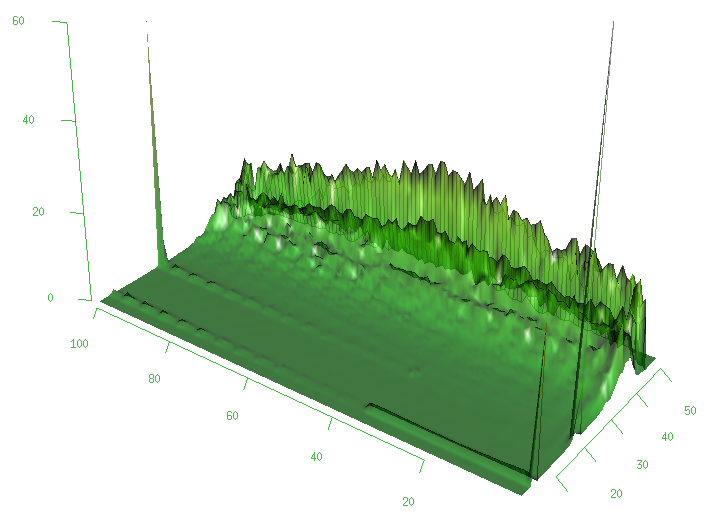
\includegraphics[width=9.5cm]{basequal_visible_cropped.png}
\end{center}
\caption{3-D Histogram of base qualities over read length for a sample BAM
  file. The x-axis (values range 1 to 100) shows the index of bases in the
  read, while the y-axis shows base quality. The z-axis is the scaled
  frequency. The plot was generated by converting the output of {\tt
    basequal\_stats.pig} using {\tt tools/basequal\_stats2matrix.pl} and then
  plotted using {\tt tools/plot\_basequal\_stats.R}.}
\label{fig:basequal3d}
\end{figure}

\subsubsection{Collecting per-base statistics of base qualities for reads}
Analogously to the previous example collecting statistics for the read bases, we can also collect
frequencies for base qualities conditioned on the position of the base inside
the reads. If these fall off too quickly for later positions, it may
indicate some quality issues with the run. The resulting script is actually
fairly similar to the previous one with the difference of not grouping
over the reference bases.
\begin{lstlisting}
A = load 'input.bam' using BamUDFLoader('yes');
B = FILTER A BY (flags/4)\%2==0 and (flags/1024)\%2==0;
C = FOREACH B GENERATE ReadSplit(name,start,read,cigar,basequal,flags,mapqual,refindex,refname,attributes#'MD');
D = FOREACH C GENERATE FLATTEN($0);
base_stats_data = FOREACH D GENERATE basepos, basequal;
base_stats_grouped = GROUP base_stats_data BY (basepos, basequal);
base_stats_grouped_count = FOREACH base_stats_grouped GENERATE group.$0 as basepos, group.$1 AS basequal, COUNT($1) AS qcount;
base_stats_grouped = GROUP base_stats_grouped_count BY basepos;
base_stats = FOREACH base_stats_grouped {
        TMP1 = FOREACH base_stats_grouped_count GENERATE basequal, qcount;
        TMP2 = ORDER TMP1 BY basequal;
        GENERATE group, TMP2;
}
STORE base_stats into 'outputfile_basequalstats.txt';
\end{lstlisting}
Here is an example output (for a BAM file with 50 reads):
\begin{lstlisting}
0       {(37,10),(42,1),(51,20),(52,1),(59,1),(61,1),(62,1),(67,2),(68,2),(70,2),(71,4),(72,3),(73,1),(75,2)}
1       {(53,1),(56,1),(61,1),(63,1),(64,1),(65,2),(67,4),(68,3),(69,2),(70,7),(71,3),(72,3),(73,1),(74,4),(75,2),(76,5),(77,6),(78,2),(80,1)}
2       {(45,1),(46,1),(51,2),(57,1),(61,1),(65,2),(66,3),(67,2),(69,3),(71,4),(72,2),(73,6),(74,7),(75,1),(76,8),(77,2),(78,3),(80,1)}
3       {(58,1),(59,1),(60,1),(61,1),(62,1),(64,1),(65,2),(67,2),(68,1),(69,5),(70,1),(71,3),(72,7),(73,2),(74,4),(75,6),(76,2),(77,4),(78,3),(79,1),(81,1)}
4       {(55,1),(60,1),(61,1),(62,1),(64,1),(66,1),(67,3),(68,2),(69,1),(70,7),(71,2),(72,1),(73,4),(74,2),(75,2),(76,2),(77,2),(78,3),(79,7),(80,4),(81,2)}
5       {(51,1),(52,2),(54,1),(58,2),(62,2),(63,1),(66,3),(68,4),(70,1),(71,1),(72,2),(73,3),(74,1),(75,8),(76,1),(77,5),(78,1),(79,6),(80,3),(81,3)}
...
\end{lstlisting}
\begin{description}
	\item[Note] This example script is equivalent to executing from the command line
\begin{lstlisting}
$ pig -param inputfile=input.bam -param outputfile=outputfile_basequalstats.txt $SEQPIG_HOME/scripts/basequal_stats.pig
\end{lstlisting}
\end{description}

\subsubsection{Filtering reads by mappability threshold}
The script {\tt filter\_mappability.pig} filters reads in a given BAM file based on a given
mappability threshold. Both input BAM and mappability file need to reside inside HDFS
\begin{lstlisting}
$ pig -param inputfile=/user/hadoop/input.bam -param outputfile=/user/hadoop/output.bam -param regionfile=/user/hadoop/mappability.100kbp.txt -param threshold=90 $SEQPIG_HOME/scripts/filter_mappability.pig
\end{lstlisting}
Note that since the script relies on distributing the bam file header and the
mappability file via Hadoop's distributed cache, it is not possible to run it
with Pig in local mode.

\subsection{Processing Qseq and Fastq data}

SeqPig supports the import and export of non-aligned reads stored in Qseq and
Fastq data. Due to Pig's model that all records correspond to tuples, which
form bags, reads can be processed in very much the same way independent
on for example whether they are stored in Qseq or Fastq.

\subsubsection{Converting Qseq to Fastq and vice versa}

The following two lines simply convert an input Qseq into Fastq.
\begin{lstlisting}
reads = load 'input.qseq' using QseqUDFLoader();
STORE reads INTO 'output.fastq' using FastqUDFStorer(); 
\end{lstlisting}
The other direction works analogously.

\subsubsection{Clipping bases and base qualities}

\label{sect:read_clipping}

Assuming there were some problems in certain cycles of the sequencer, it
may be useful to clip bases from reads. This example removes the last 3
bases and their qualities and stores the data under a new filename. Note
that here we rely on the {\tt SUBSTRING} and {\tt LENGTH} string functions, which is
part of the PiggyBank (see Section~\ref{sect:piggybank_note}).

\begin{lstlisting}
DEFINE SUBSTRING org.apache.pig.piggybank.evaluation.string.SUBSTRING();
DEFINE LENGTH org.apache.pig.piggybank.evaluation.string.LENGTH();
reads = load 'input.qseq' using QseqUDFLoader();
B = FOREACH A GENERATE instrument, run_number, flow_cell_id, lane, tile, xpos, ypos, read, qc_passed, control_number, index_sequence, SUBSTRING(sequence, 0, LENGTH(sequence) - 3) AS sequence, SUBSTRING(quality, 0, LENGTH(quality) - 3) AS quality;
store B into 'output.qseq' using QseqUDFStorer();
\end{lstlisting}
\begin{description}
	\item[Note] This example script is equivalent to executing from the command line
\begin{lstlisting}
$ pig -param inputfile=input.qseq -param outputfile=output.qseq -param backclip=3 $SEQPIG_HOME/scripts/clip_reads.pig
\end{lstlisting}
\end{description}

\section{Further information}

\subsection{Hadoop parameters}

Some scripts (such as {\tt pileup2.pig}) require an amount of memory that
depends on the choice of command line parameters. To tune the performance of
such operations on the Hadoop cluster,
consider the following Hadoop-specific parameters in {\tt mapred-site.xml}.
\begin{itemize}
\item {\tt mapred.tasktracker.map.tasks.maximum}: \\the maximum number simultaneous map tasks per worker node
\item {\tt mapred.tasktracker.reduce.tasks.maximum}:\\ the maximum number simultaneous reducer tasks per worker node
\item {\tt mapred.child.java.opts}:\\ Java options passed to child virtual
	machines at the worker nodes; for instanced, this may be used to configure
	the Java heap size to 1GB with {\tt -Xmx1000M}
\end{itemize}
Additionally, it is possible to pass command line parameters (such as mapper and reducer memory limits).
For instance, consider the Pig invocation (see {\tt tools/tun\_all\_pileup2.sh})
\begin{lstlisting}
${PIG_HOME}/bin/pig -Dpig.additional.jars=${SEQPIG_HOME}/lib/hadoop-bam-5.0.jar:${SEQPIG_HOME}/build/jar/SeqPig.jar:${SEQPIG_HOME}/lib/seal.jar:${SEQPIG_HOME}/lib/picard-1.76.jar:${SEQPIG_HOME}/lib/sam-1.76.jar -Dmapred.job.map.memory.mb=${MAP_MEMORY} -Dmapred.job.reduce.memory.mb=${REDUCE_MEMORY} -Dmapred.child.java.opts=-Xmx${CHILD_MEMORY}M -Dudf.import.list=fi.aalto.seqpig -param inputfile=$INPUTFILE -param outputfile=$OUTPUTFILE -param pparallel=${REDUCESLOTS} ${SEQPIG_HOME}/scripts/pileup2.pig
\end{lstlisting}
By setting appropriate values for {\tt MAP\_MEMORY, REDUCE\_MEMORY,
CHILD\_MEMORY} and for the number of available reduce slots {\tt REDUCESLOTS}
one may be able to improve performance.

\subsection{Compression}

For optimal performance and space usage it may be advisable to enable the compression of
Hadoop map (and possible reduce) output, as well as temporary data generated
by Pig. Compression with Pig can be enabled by setting properties such as
\begin{lstlisting}
  -Djava.library.path=/opt/hadoopgpl/native/Linux-amd64-64
  -Dpig.tmpfilecompression=true -Dpig.tmpfilecompression.codec=lzo
  -Dmapred.output.compress=true
  -Dmapred.output.compression.codec=org.apache.hadoop.io.compress.GzipCodec
\end{lstlisting}
on the Pig command line or the Hadoop configuration. Note that currently not all
Hadoop compression codecs are supported by Pig.  The details regarding which
compression codec to use depend are beyond the scope of this manual.
